As shown in Figure ~\ref{fig:diffusion_plot_a}, diffusion analysis demonstrated that Alexa Fluor conjugated antibodies exhibited significantly higher diffusion coefficients and shorter diffusion times compared to IRDye conjugated antibodies. Specifically, anti-CD80 labeled with AF700 and
anti-PDL1 labeled with AF750 had diffusion coefficients of $(9.00 \pm 0.27) \times 10^{-7} \mathrm{cm}^2/\mathrm{s}$ and ($8.35 \pm 0.26) \times 10^{-7} \mathrm{cm}^2/\mathrm{s}$, respectively. In contrast, anti-PD1 labeled with IR680 and the untargeted IgG control labeled with IR800 had lower diffusion coefficients of ($5.47 \pm 0.48) \times 10^{-7} \mathrm{cm}^2/\mathrm{s}$ and
($4.93 \pm 0.77) \times 10^{-7} \mathrm{cm}^2/\mathrm{s}$, respectively. As a result, Alexa Fluor conjugated agents diffused through the $10.6$ mm agarose phantom more rapidly, reaching near-equilibrium conditions within $55.3 \pm 0.14$ minutes for anti-CD80 and $56.6 \pm 1.8$ minutes for anti-PDL1. In contrast, the IRDye-labeled agents had longer diffusion times, with anti-PD1 reaching equilibrium at $86.20 \pm 7.8$ minutes and IgG control at 99.7 ± 14 minutes. Based on these results, a standardized incubation period of 120 minutes was adopted for all subsequent mPAI imaging experiments of tissue-mimicking phantoms with cells.

As shown in Figure ~\ref{fig:diffusion_plot_b}, the difference between the diffusion coefficients of the free dye IR680, ($4.93  \pm 0.0017)\times 10^{-6} \mathrm{cm}^2/\mathrm{s}$, and the soluble PD1 conjugated to IR800, ($1.16 \pm 0.0027) \times 10^{-6} \mathrm{cm}^2/\mathrm{s}$, is not statistically significant. Their diffusion times were $34.2 \pm 4.0$ minutes and $42.2 \pm 9.8$ minutes, respectively. Based on these results, a 60-minute incubation period was established for the PAI experiments using soluble PD1. A summary of these data is provided in Table ~\ref{tab:diffusion_summary}.

\begin{table}[H]
    \centering
    \caption{Summary of mean diffusion coefficients and diffusion times}
    \label{tab:diffusion_summary}
    \begin{tabular}{l|c|c}
        \hline
        \multirow{2}{*}{\textbf{Imaging Agent}} &
        \multicolumn{2}{c}{\textbf{Mean (standard deviation)}} \\
        \cline{2-3}
        & \textbf{Diffusion Coefficient} ($\mathrm{cm}^2/\mathrm{s}$) & \textbf{Time (mins)} \\
        \hline
        anti-PDL1-AF750       & $(8.35 \pm 0.26) \times 10^{-7}$  & $56.6 \pm 1.8$ \\
        \hline
        anti-PD10IR680        & $(5.47 \pm 0.48) \times 10^{-7}$  & $86.2 \pm 7.8$ \\
        \hline
        anti-CD80-AF700       & $(9.00 \pm 0.27) \times 10^{-7}$  & $55.3 \pm 1.4$ \\
        \hline
        anti-IgG-IR800        & $(4.93 \pm 0.77) \times 10^{-7}$  & $99.7 \pm 14.0$ \\
        \hline
        IR800 (free dye)      & $(4.93 \pm 0.017) \times 10^{-6}$ & $34.2 \pm 4.0$ \\
        \hline
        Soluble PD1-IR800     & $(1.16 \pm 0.027) \times 10^{-6}$ & $42.2 \pm 9.8$ \\
        \hline
    \end{tabular}
\end{table}

\begin{figure}[H]
    \centering
    \begin{minipage}{0.85\linewidth}
        \centering
        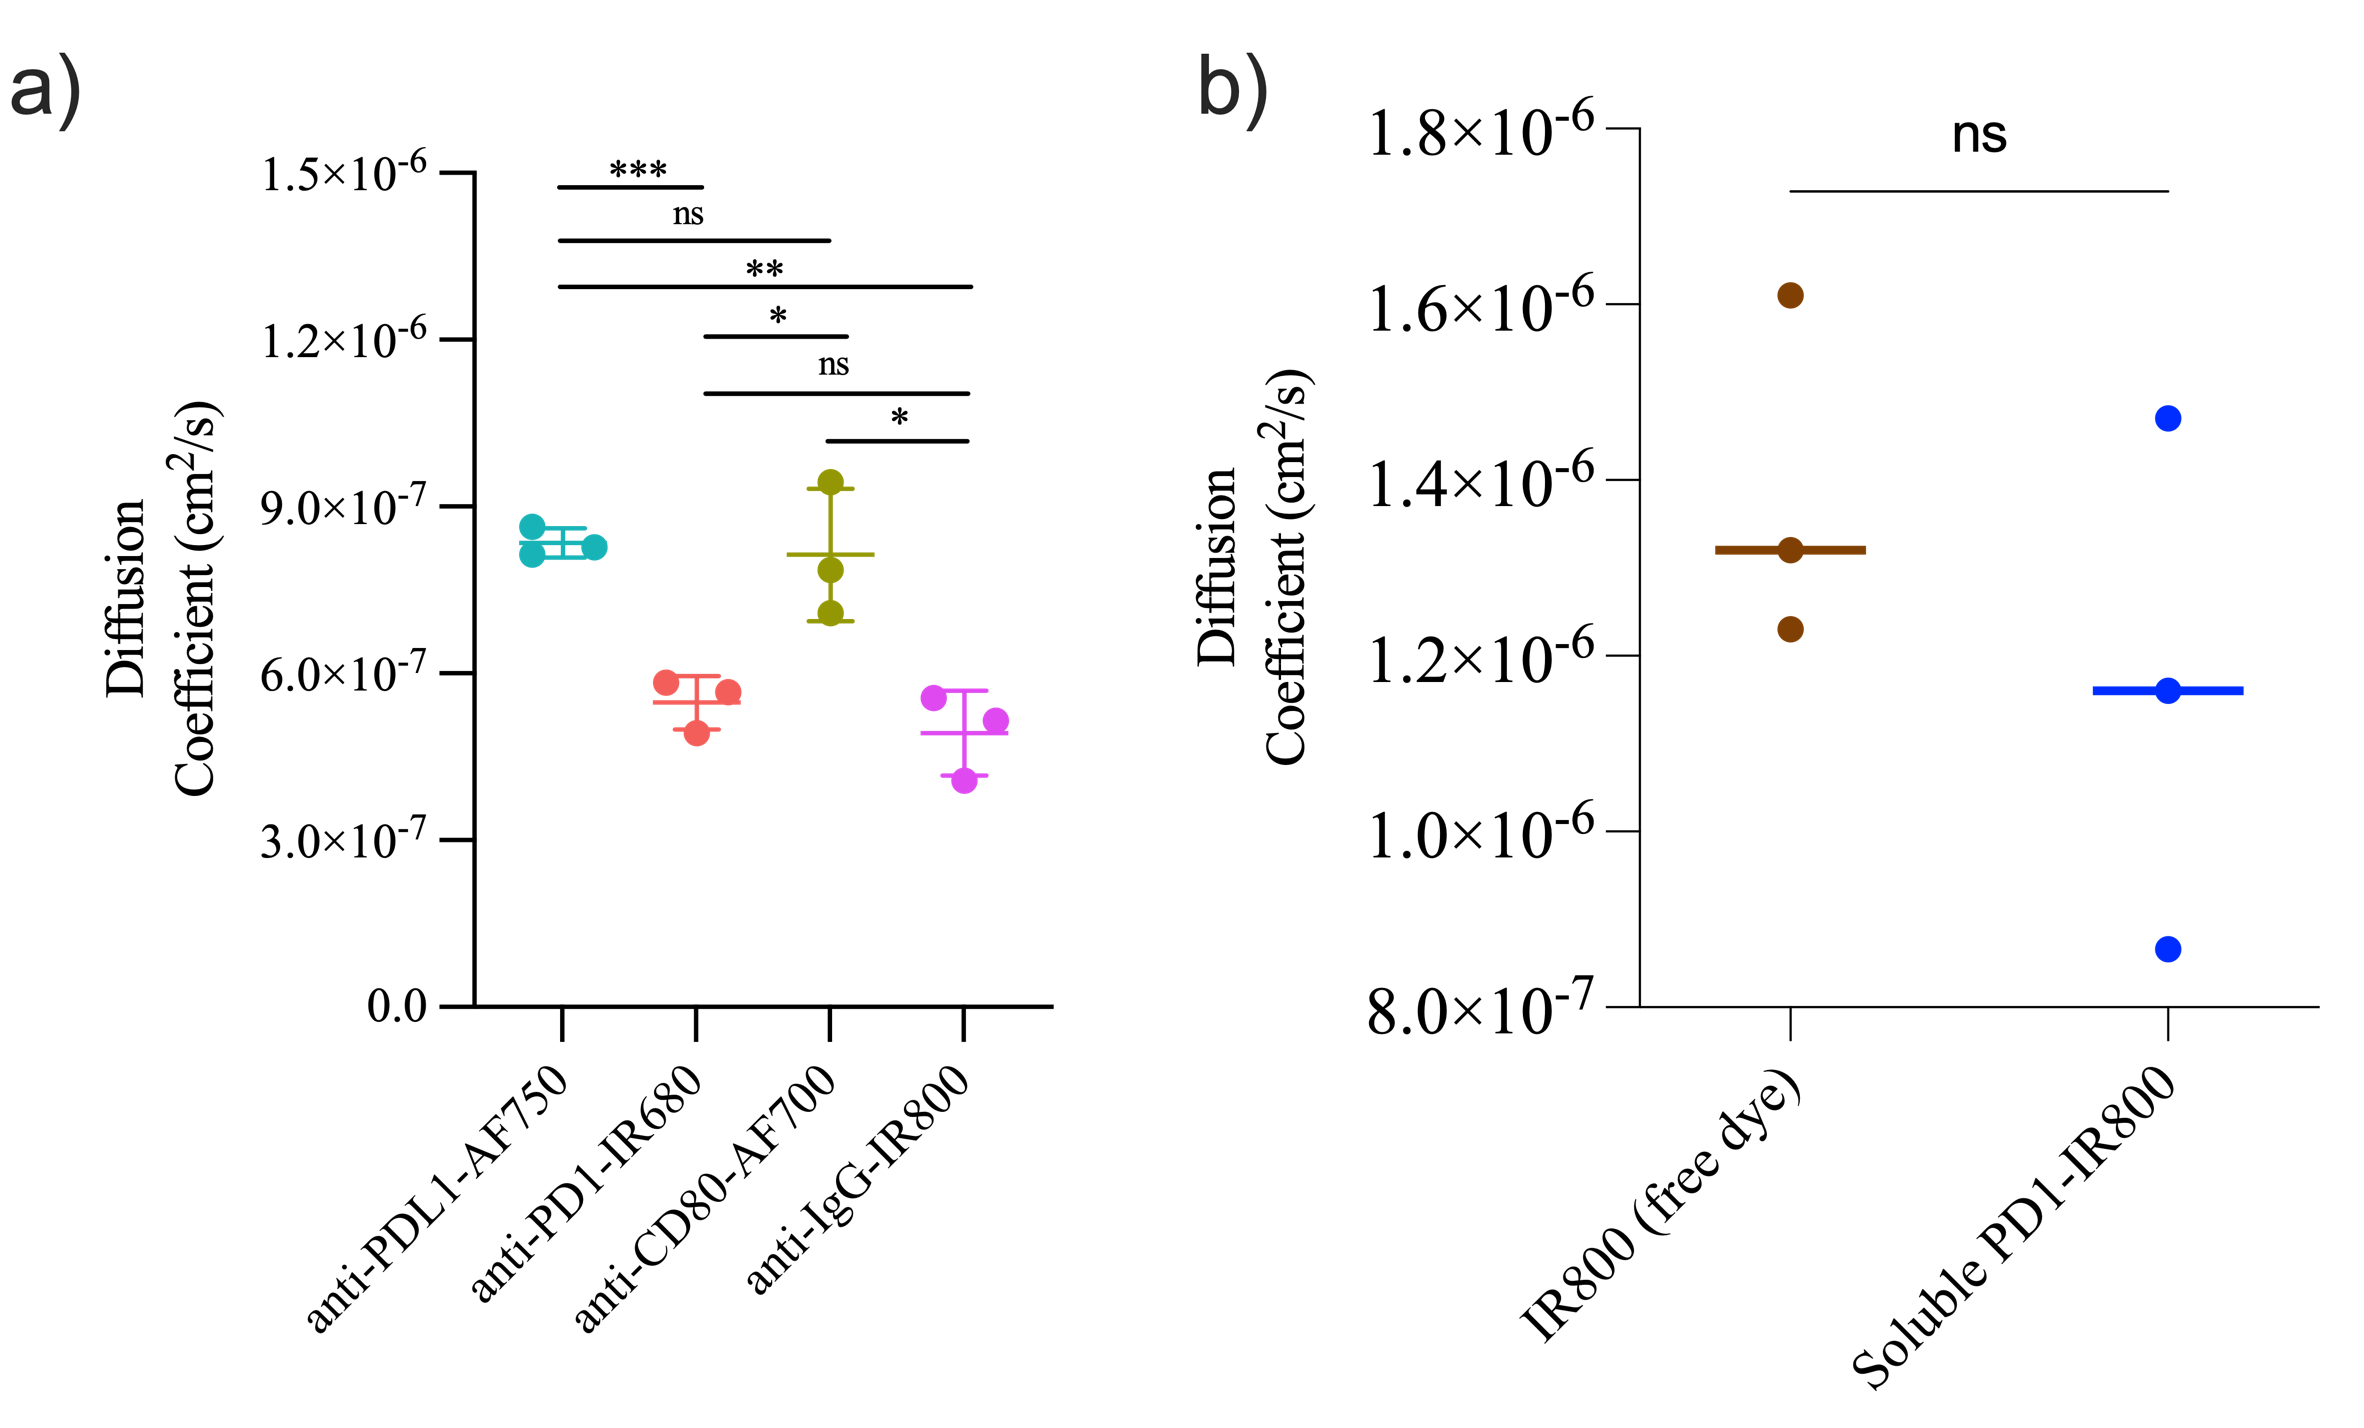
\includegraphics[width=\linewidth]{figures/diffusion_plots.png}

        % Phantom labels for subfigure referencing
        \begin{minipage}{0pt}
            \phantomsubcaption\label{fig:diffusion_plot_a}
            \phantomsubcaption\label{fig:diffusion_plot_b}
        \end{minipage}

        \captionsetup{justification=raggedright, singlelinecheck=false}
        \caption[Comparison of diffusion coefficients]{\textbf{Comparison of the Diffusion Coefficients of Different Imaging Agents.}
        (a) Distribution of diffusion coefficients for antibodies conjugated to fluorophores. Alexa Fluor-conjugated antibodies 
        (PDL1-AF750 and CD80-AF700) exhibited significantly higher diffusion coefficients compared to IRDye-conjugated antibodies (PD1-IR680 and 
        IgG-IR800). (b) Distribution of diffusion coefficients for free IR800 dye and soluble PD1-IR800. Asterisks indicate statistically significant 
        differences, while “ns” denotes non-significant differences.}
        \label{fig:diffusion_plots}
    \end{minipage}
\end{figure}
